%% This is an example first chapter.  You should put chapter/appendix that you
%% write into a separate file, and add a line \include{yourfilename} to
%% main.tex, where `yourfilename.tex' is the name of the chapter/appendix file.
%% You can process specific files by typing their names in at the 
%% \files=
%% prompt when you run the file main.tex through LaTeX.
\chapter{Metatranscriptome analyses indicate resource partitioning between diatoms in the field}
\raggedbottom
%\begin{singlespace}
%Harriet Alexander$^{1,2}$, Bethany D. Jenkins$^{3,4}$, Tatiana A. Rynearon$^{3}$, Sonya T. Dyhrman$^{5}$\\
%\\
%$^{1}$ MIT-WHOI Joint Program in Oceanography/Applied Ocean Science and Engineering, Cambridge, MA 02139, USA\\
%$^2$ Biology Department, Woods Hole Oceanographic Institution, Woods Hole, MA 02543, USA\\
%$^3$ Graduate School of Oceanography, University of Rhode Island, Narragansett, RI 02882, USA\\
%$^4$ Department of Cell and Molecular Biology, University of Rhode Island, Kingston, RI 02881, USA\\
%$^5$ Department of Earth and Environmental Sciences Lamont-Doherty Earth Observatory, Columbia University, Palisades, NY 10964\\
%\\
\let\thefootnote\relax\footnotetext{This chapter was originally published as Alexander, H., Jenkins, B.D., Rynearson, T.A., and Dyhrman, S.T. (2015). \href{http://www.pnas.org/content/112/17/E2182.long}{Metatranscriptome analyses indicate resource partitioning between diatoms in the field}. \emph{Proc. Natl. Acad. Sci. U. S. A.} 112:17, E2182-E2190.}
\let\thefootnote\relax\footnotetext{H.A., B.D.J., T.A.R., and S.T.D. designed research; H.A., B.D.J., T.A.R., and S.T.D. performed research; H.A. contributed new reagents/analytic tools; H.A. analyzed data; and H.A., B.D.J., T.A.R., and S.T.D. wrote the paper.}

%\end{singlespace}
\clearpage
\section{Abstract}
Diverse communities of marine phytoplankton carry out half of global primary production. The vast diversity of the phytoplankton has long perplexed ecologists, as these organisms coexist in an isotropic environment while competing for the same basic resources (e.g. inorganic nutrients). Differential niche partitioning of resources is one hypothesis to explain this ``paradox of the plankton,'' but it is difficult to quantify and track variation in phytoplankton metabolism \textit{in situ}. Here we use quantitative metatranscriptome analyses to examine pathways of nitrogen (N) and phosphorus (P) metabolism in diatoms that co-occur regularly in an estuary on the east coast of the US (Narragansett Bay). Expression of known N and P metabolic pathways varied between diatoms, indicating apparent differences in resource utilization capacity that may prevent direct competition.  Nutrient amendment incubations skewed N:P ratios, elucidating nutrient responsive patterns of expression, and facilitating a quantitative comparison between diatoms. The resource-responsive (RR) gene sets deviated in composition from the metabolic profile of the organism, being enriched in genes associated with N and P metabolism. Expression of the RR gene set varied over time and differed significantly between diatoms, resulting in opposite transcriptional responses to the same environment. Apparent differences in metabolic capacity and the expression of that capacity in the environment suggest that diatom-specific resource partitioning was occurring in Narragansett Bay. This high-resolution approach highlights the molecular underpinnings of diatom resource utilization and how co-occurring diatoms adjust their cellular physiology to partition their niche space. 
 
\section{Introduction}
The stability and primary productivity of ecosystems has long been linked to the diversity of primary producers \citep{Elton1958, Cardinale2012}. This is well documented in terrestrial systems \citep{Naeem1994, Tilman2001, Cadotte2013, Balvanera2006, Tilman1996} and is increasingly being established for marine systems \citep{Behl2011, Striebel2009, Steiner2005, Ptacnik2008}. Marine phytoplankton generate roughly half of global primary production \citep{Nielsen1960, Strickland1965, Field1998} and play a critical role in oceanic ecosystem structure and function. Within the phytoplankton, the diatoms generate an estimated 40\% of primary production \citep{Nelson1995}. Thus diatoms alone exert profound influence over marine primary production and global carbon (C) cycling, particularly in coastal margins and estuaries. \par
Phytoplankton are extremely diverse, with estimates of over 200,000 extant species \citep{Sournia1991, Tett1995, Mann1996}. This dramatic level of taxonomic diversity in the plankton is difficult to resolve with the apparently limited number of niches in the pelagic habitat, as these organisms compete for the same two basic resources: light and nutrients. As was highlighted by \citet{Hutchinson1961}, the phytoplankton violate Gause's law of competitive exclusion, which posits that two organisms competing for the same resources cannot coexist. Much thought has gone towards identifying the cause of the ``paradox of the plankton'' and include explanations such as ``contemporaneous disequilibrium'' of patchy phytoplankton distributions \citep{Richerson1970}, life history differences \citep{Huisman2001}, species oscillations \citep{Huisman1999}, environmental fluctuation \citep{Roy2007}, intra-specific variation \citep{Menden-deuer2014}, and differential niche partitioning \citep{Connel1980}. Of these potential factors, one of the most difficult to directly observe in the plankton is niche partitioning. Different species may have unique strategies that allow them to specialize on certain resources or nutrient forms, and species may have different responses to resource shifts that allow them to avoid competition. Such specialization in eco-evolutionary strategy may underlie the ``winner-loser'' dynamics observed in productive estuaries and coastal systems, yet resolving patterns of species-specific resource metabolism in the field remains a central challenge.\par
It is accepted that the macronutrients N and P are central to the structuring of phytoplankton communities across large spatial and temporal scales \citep{Margalef1963, Follows2007, Johnson2006b}, and that phytoplankton compete for nutrients in the natural environment \citep{Sommer1983, Sommer1985}. Studies focused on nutrient geochemistry, and phytoplankton quotas or uptake have emphasized the importance of nutrients to community dynamics, but these do not generally examine resource partitioning between individual species \citep{Hutchins1999, Zubkov2003}. Transcriptional studies provide species-specific resolution, but few studies have examined the global expression of nutrient metabolism pathways in the field \citep{Marchetti2012a} or in organisms lacking a fully sequenced genome \citep{Frischkorn2014, Moustafa2010}, and as a result, the mechanistic underpinnings of phytoplankton resource metabolism \textit{in situ} are not well understood. In situ global gene expression analyses (metatranscriptome profiling) are a means for elucidating a species' metabolic capacity and examining patterns in resource utilization potential through time by tracking the expression of species' resource-responsive genes. When simultaneously applied to multiple species in a sample, this can resolve differences in the expressed gene compliment and how it is modulated, which may reflect resource partitioning of phytoplankton niche space \citep{Gifford2013}. For example, this approach has uncovered species-specific expression of genes for the transport of organic compounds \citep{Poretsky2010, Rinta-Kanto2012a, Gifford2011}, highlighting potential differences in resource partitioning. Although increasingly critical for identifying resource utilization in the bacterioplankton, metatranscriptome profiling has only recently been used to examine resource utilization in coastal eukaryotic phytoplankton populations \citep{Dupont2015}, largely due to challenges in quantifying a transcriptional response in a mixed population and until recently, the lack of reference genomes and transcriptomes for determining the origin of the transcriptional response. Co-occurring phytoplankton may possess different metabolic capabilities and responses to resource availability, which may then enable resource partitioning and the segregation of the fundamental niche or the realized niche. Knowledge of if and how these organisms modulate their niche space would allow predictive models to better resolve species distribution and ecosystem structure and function in the future ocean \citep{Follows2007}.\par
Herein we examined pathways of resource metabolism between two co-occurring diatoms from the genera \textit{Thalassiosira} and \textit{Skeletonema}, sampled from a time-series site in Narragansett Bay. Narragansett Bay is a highly productive and dynamic estuarine environment on the east coast of the United States with an estimated bay-wide average net production of $269\ gC\ m^{2}\ yr^{-1}$ \citep{Oviatt1981}. Quantitative metatranscriptomic techniques were developed and used to: 1) assign taxonomic designation, 2) assess and track changes in known metabolic capacity through quantitative molecular fingerprinting (QMF), 3) statistically identify the resource responsive gene set, and 4) proportionalize the expression of resource-responsive genes to track species-specific responses through time, using standardized transcriptional differentiation scores ($STD$). This multifaceted computational approach enabled the unprecedented resolution of the unique strategies these two diatoms use for resource acquisition. \par
\section{Materials and Methods}
\subsection{Experimental set up and sample collection}
Surface seawater was collected and sampled for total community RNA at the long-term sampling site in Narragansett Bay, RI ($41^\circ 34^\prime 07^{\prime \prime}$ N, $71^\circ 23^\prime 31^{\prime \prime}$ W) during 2012 (16 May, 21 May, 30 May, 4 June, and 8 June, here called S1 through S5) in conjunction with the weekly time-series sampling effort. To diminish the influence of diel signals, samples were collected and processed between 0830 and 0900 local time. Near surface water was collected in an acid-washed carboy and then filtered onto polycarbonate filters (5.0 $\mu$m pore size, 47mm) using a peristaltic pump. Filters were then placed in cryovials and stored in liquid nitrogen until RNA extraction. In this manner all samples were preserved within 15 minutes of collection. In addition to sampling for total community RNA, phytoplankton abundance was measured as part of the long-term weekly survey \citep{Furnas1983, Furnas1982}.\par
A nutrient amendment incubation experiment was performed on 30 May 2012, with S3 representing the t = 0 of the experiment. Water collected in conjunction with S3 was pre-filtered through 200µm mesh to remove large zooplankton grazers and placed into acid washed 2.5 L bottles. Triplicate bottles were then amended with nutrients to create five treatments: +N, +P, -N, -P, and ambient control. The +N and +P treatments were designed to eliminate the N and P stress signals, respectively, while the -N and -P treatments were supplemented with everything except the nutrient in question (e.g. the -N treatment was amended with P, Si, Fe, and vitamins), to force the draw down of N and P, respectively (Table \ref{tab:a3t2}). N and P amendment concentrations were selected to be approximately 10x the seasonal average ambient N and P concentrations in the surface waters of Narragansett Bay measured at Station II. Silica, Fe, and f/5 vitamin amendments were made in proportion to the f/5 media ratios \citep{Guillard1975}. Bottles were placed in a flow-through incubator at ambient temperatures and PAR to mimic the collection depth. The incubation was run for 48 hours, at which point all treatments were sampled for total community RNA as described above by filtering and snap- freezing 2L of biomass from each replicate bottle. \par
\subsection{RNA extraction and sequencing}
Filters from triplicate bottles, representing approximately 6 L of water, were pooled by treatment and extracted for each of the \textit{in situ} and incubation experiment samples. RNA was extracted from individual filters with the RNAeasy Mini Kit (Qiagen), following a modified version of the yeast protocol. Briefly, lysis buffer and RNA-clean zircon beads were added to the filter and samples were vortexed for 1 minute, placed on ice for 30 seconds, and then vortexed again for 1 minute. Samples were then processed following the yeast protocol. The resulting RNA was eluted in water and then treated for possible DNA contamination using TURBO DNA-free Kit (Ambion) following the Rigorous Dnase protocol. RNA from each triplicate was then pooled by sample or treatment, using the RNA Cleanup Protocol from the RNAeasy Mini Kit (Qiagen). The total RNA ( $>1000$ ng for each sample) was then enriched for eukaryotic mRNA through a poly-A pull down onto oligo-dT beads. The resulting enriched RNA sample then went through library preparation with the Illumina TruSeq RNA Prep Kit (Illumina). Libraries were sequenced at the Columbia University Genome Center (New York, New York) with an Illumina HiSeq2000. Each sample was sequenced to produce ~ 60 million, 100 base pair, paired end reads (Table \ref{tab:a3t1}). Raw sequence data quality was visualized using FastQC \citep{Andrewsa} and then cleaned and trimmed using Trimmomatic v 0.27 (paired end mode; 6-base pair wide sliding window for quality below 20; minimum length 25 base pair) \citep{Lohse2012}. Environmental sequence reads are available at the NCBI under accession number \href{http://www.ncbi.nlm.nih.gov/sra/?term=SRP055134}{SRP055134}. 
\subsection{Transcriptome and genome mapping}
To assign taxonomic identification to the reads a database was created from transcriptomes made publicly available as of 17 March 2014 through the Marine Microbial Eukaryote Transcriptome Sequencing Project (MMETSP). In total, 401 transcriptomes from 209 species or cultured isolates were collected. Like-species transcriptomes were combined (regardless of strain or condition) using CD-HIT-EST (98\% identity; word size of 9). The resulting clustered set of transcripts was considered to be the representative transcriptome for the species or cultured isolate. The 209 transcriptomes created in this manner were concatenated to form a comprehensive species-level transcriptome database from the MMETSP library. Due to the large size of the resulting MMETSP database, trimmed reads were mapped to the MMETSP using the Burrows-Wheeler Aligner (BWA) \citep{Li2010} and then counted using the HTSeq 0.6.1 package \citep{Anders2014}.\par 
Transcriptomes from two ecologically relevant diatom species in Narragansett Bay were selected: \textit{Skeletonema} costatum RCC1716 (MMETSP0013, accessed from the publicly available transcriptome databases, Moore Foundation Marine Microbiology Initiative-supported Marine Microbial Eukaryote Transcriptome Sequencing Project, National Center for Genome Resources) and \textit{Thalassiosira rotula} CCMP3096 (a custom assembly available at EBI, accession number Hx2000045970). These transcriptomes were individually clustered using CD-HIT-EST (parameters: -c 0.98, -n 9) \citep{Li2006}. The resulting clustered set of transcripts was then concatenated to form a reference transcriptome database. Trimmed reads from the field and incubation samples were mapped to this transcriptome database using Bowtie2 v 2.2.1 (parameters: -a –sensitive) \citep{Langmead2012}. As a point of comparison, reads were also mapped using Bowtie2 v2.2.1 under the same parameters to the genome of the model centric diatom species, Thalassiosira pseudonana CCMP1335 (v3.0), an organism not known to be abundant in Narragansett Bay. Mapped reads were then counted by transcript using the HTSeq 0.6.1 python package (parameters: -m union –s no) \citep{Anders2014}. Reads aligning to more than one full transcript were not counted. KEGG pathways were assigned to the assembled sequences using the online KEGG Automatic Annotation Server (KAAS), using the bi-directional best-hit (BBH) method to obtain KEGG Orthology annotations. In this study, only genes with a normalized count (NC) (raw count / total number of genes mapped to an organism) of at least 2 tags per million (TPM) in at least one of the field or incubation samples were included, thus limiting the sample set to 4318 genes for \textit{T. rotula} (19.3\% of the transcriptome) and 20921 genes for \textit{Skeletonema} spp. (75.6\% of the transcriptome). This difference in coverage is directly related to their relative abundance in the population.
\subsection{Transcriptome clustering}
To assess relatedness of genes within \textit{Skeletonema} spp. and \textit{T. rotula}, the transcriptomes were translated using \href{http://proteomics.ysu.edu/tools/OrfPredictor.html}{ORF Predictor} using a reference BLASTx alignment against the NCBI database with an 1e-5 cutoff \citep{Min2005}. These translated peptide sequences were then combined with the translated proteins from the diatom genomes \textit{Fragilariopsis cylindrus} CCMP1102 v1.0, \textit{Phaeodactylm tricornutum} CCMP632 v2.0, \textit{Pseudo-nitzschia multiseries} CLN-47 v1.0, and \textit{Thalassiosira pseudonana} CCMP1335 v3.0, which were collected from the Joint Genome Institute \href{http://genome.jgi-psf.org}{JGI} database. A protein similarity network was then created using EGN, a software program that automates the reconstruction of gene networks from protein sequences through reciprocal BLASTp analysis (e-value <1e-5, hit identity threshold: 20\%, best-reciprocal threshold of best e-value: 5\%, minimal match coverage threshold: 90\%) \citep{Halary2013, Halary2010}. Networks were then visualized and manipulated using Cytoscape 3.0, where the layout of the network was produced using an edge-weighted spring-embedded model based on e-value, meaning that genes that are closer together are more similar \citep{Smoot2011, Saito2012}. Known RR genes from previous transcriptome studies of the diatom species, \textit{T. pseudonana}, were selected for analysis: 1) the P-responsive gene, Thaps\_24435, a NPT \citep{Dyhrman2012} and 2) the N-responsive gene, Thaps\_25299, an assimilatory nitrate reductase \citep{Bender2014}. 
\subsection{Identification of stable and nutrient-responsive genes}
Intercomparison of nutrient-incubation experiments enabled the identification of both nutrient-responsive genes and stably expressed reference genes for \textit{T. rotula} and \textit{Skeletonema} spp.. For each organism, RR genes were identified by comparing the counts for that organism in +N to the -N incubation and the +P to the -P incubation, respectively, using Analysis of Sequence Counts (ASC), an empirical Bayes method, which estimates the prior distribution from the data, itself \textit{Wu2010}. ASC analyses were run using raw count data from each species separately. Genes were considered to be differentially regulated between treatments if for a fold change of 2.0 the posterior probability (post-$p$) was greater than 0.95 \citep{Dyhrman2012}. After surveying the output of several different post-$p$ cutoffs (Figure \ref{fig:a3f11}), stable genes were identified using ASC as described by \citet{Alexander2012} through pairwise comparisons of each of the incubation treatments (fold change of 1.25, post-$p < 0.1$). 
\subsection{Normalization of metatranscriptome data}
Counts from the field were first normalized to the sequences belonging to the species in the library (Equation \ref{eq:NC}). For a particular species, $c$, the number of reads mapping to a gene $g$, $c_{i,g}$, was normalized to the sum of all the counts across all genes for that organism yielding the normalized count, $NC_{i,g}$, similar to normalization techniques used for metatranscriptome data \citep{Marchetti2012a, Ottesen2011}. 
%Equation 1. Normalized counts
\begin{equation}
	\label{eq:NC}
	NC_{i,g} = \frac{c_{i,g}}{\sum \limits_{g \epsilon G} c_{i,g}}
\end{equation}

From hence forth, only genes for which $NC > 2$ TPM in at least one sample (incubation or field) were considered. To facilitate interspecies comparisons, the NC was normalized to the geometric mean of the set of stable reference genes, $R$, yielding a stable gene normalized count ($SGNC$). The calculation of $SGNC$ (Equation \ref{eq:SGNC}) for transcriptome data, while a novel application to metatranscriptome analysis, was designed to emulate the normalization used in qRT-PCR studies \citep{Vandesompele2002}. \par
%Equation 2. Stable gene normalized counts
\begin{equation}
	\label{eq:SGNC}
 	SGNC_{i,g}=\frac{NC_{i,g}}{\left ( \prod \limits^{R} NC_{i,g} \right ) ^{1/R}}
\end{equation}

The nutrient responsive genes identified as differentially expressed in the nutrient incubations (Table \ref{tab:a3t2}) were then selected for investigation in the field metatranscriptomes (S1 through S5). The $SGNC$ from the field for these nutrient-related genes were bounded by the $SGNC$ from like nutrient incubations to calculate the standardized transcriptional differentiation score for N ($STD_N$) (Equation \ref{eq:STDN}) and P ($STD_P$) (Equation \ref{eq:STDP}).\par 

%Equation 3. Standardized transcriptional differentiation score (nitrogen)
\begin{equation}
	\label{eq:STDN}
	STD_N = \frac{SGNC_{field} - SGNC_{+N}}{SGNC_{-N} - SGNC_{+N}} 	
\end{equation}

%Equation 4. Standardized transcriptional differentiation score (phosphorus)
\begin{equation}
	\label{eq:STDP}
	STD_N = \frac{SGNC_{field} - SGNC_{+P}}{SGNC_{-P} - SGNC_{+P}} 	
\end{equation}

For example, in calculating $STD_N$, the $SGNC_{field}$ is put in the range of the $SGNC_{+N}$ and $SGNC_{-N}$. By consequence, if the $STD_N$ for a gene in the field equals zero it is more similar in expression to the +N treatment and if it equals one it is more similar in expression to the -N treatment. As such, a plot $STD_N$ against $STD_P$, can divide the space into two main theoretical quadrants N:P > Redfield ($STD_P > 1$ and $STD_N < 0$) and N:P < Redfield ($STD_N > 1$ and $STD_P < 0$) (Figure \ref{fig:a3f8}). The total number of genes falling into each of the quadrants were counted by varying the bounds considered: the N:P > Redfield ratio quadrant ($STD_P > C$; $STD_N < C$, for $0.25 < C < 0.75$) and the N:P < Redfield ratio quadrant ($STD_P < C$; $STD_N > C$, for $0.25 < C < 0.75$). To conservatively approximate variation, the value of C was varied over 10 different values and the average and standard deviation for the percentages of genes falling into each of the quadrants was quantified. Similarity of data between species by quadrant was assessed using an analysis of variance (ANOVA) with a generalized linear model. The results from a post hoc Tukey test show the divergence of species across time ($p < 0.05$).

\section{Results and Discussion}
\subsection{Samples and sequencing}
Narragansett Bay has seasonal blooms of diatoms which have been monitored through weekly cell counts for over 50 years at a long-term time series station \citep{Borkman2009, Li1998}. Five eukaryotic surface metatranscriptome samples were taken from surface seawater collected during May and June of 2012 at the time-series site yielding over 358 million 100 base pair, paired end cDNA reads from the field (S1-5) (Table \ref{tab:a3t1}). In conjunction with these field-based surveys, a nutrient amendment incubation experiment was performed with natural communities on 30 May 2012 (S3) to drive the community towards opposite extremes in the nitrogen (N): phosphorus (P) ratio (Redfield ratio) (Table \ref{tab:a3t2}). Eukaryotic metatranscriptomes from the five incubation treatments produced over 264 million 100 base pair, paired end cDNA reads (Table \ref{tab:a3t1}).\par

To assign taxonomic designation, sequences from the time series were conservatively mapped (such that if a read mapped to more than one gene it was discarded) to a sequence library containing all assembled sequences and annotations generated through the Marine Microbial Eukaryotic Transcriptome Sequencing Project (MMETSP) \citep{Keeling2014} which were public as of 17 March 2014. The custom sequence library contained 401 transcriptomes across 209 species or cultured isolates. Between 62 to 71\% of reads from the \textit{in situ} samples mapped to the MMETSP database with diatoms dominating the libraries, representing 30 to 46\% of the total mapped reads (Figure \ref{fig:c3f1}). The peak in diatom representation coincided with a bloom of \textit{Skeletonema} spp. detected in time-series cell counts (Figure \ref{fig:a3f1}), and a period of historical overlap between the \textit{Skeletonema} and \textit{Thalassiosira} genera. \textit{Skeletonema} and \textit{Thalassiosira} were well represented during the time period studied in both mapped RNA (Figure \ref{fig:c3f1}) and cell counts (Figure \ref{fig:a3f1}). \textit{T. rotula} was present but at low abundance during the time-series, while \textit{Skeletonema} spp. was abundant, with sampling spanning a bloom of \textit{Skeletonema} (>10,000,000 cells L$^{-1}$), with peak cell densities in S2 (21 May 2012) (Figure \ref{fig:a3f1}). As such, subsequent analyses were focused on these two groups by remapping the data to representative transcriptomes: \textit{T. rotula} and \textit{S. costatum} (Table \ref{tab:a3t1}). \textit{S. costatum} was chosen as it was the transcriptome from the genus \textit{Skeletonema} that recruited the most hits in the MMETSP database. Because \textit{Skeletonema} is known to include morphologically cryptic species that can only be identified by scanning electron microscopy \citep{Sarno2005, Zingone2005, Smayda2011}, it is referred to here as \textit{Skeletonema} spp. for clarity. Up to 17.5 and 54.9\% of reads from a single sample mapped to \textit{T. rotula} and \textit{S. costatum}, respectively. As a point of comparison, reads were also mapped to the genome of a second Thalassiosirid, \textit{T. pseudonana}, a diatom that is not known to be abundant in Narragansett Bay (Table \ref{tab:a3t1}). Though displaying high identity with the 18S rDNA to \textit{T. rotula} and \textit{S. costatum} (96\% and 93\% identity, respectively), less than 1\% of the metatranscriptome reads mapped \textit{T. pseudonana} (Table \ref{tab:a3t1}), highlighting the specificity of the approach. 

% Figure 1
\begin{figure}[h!]
  \centering
    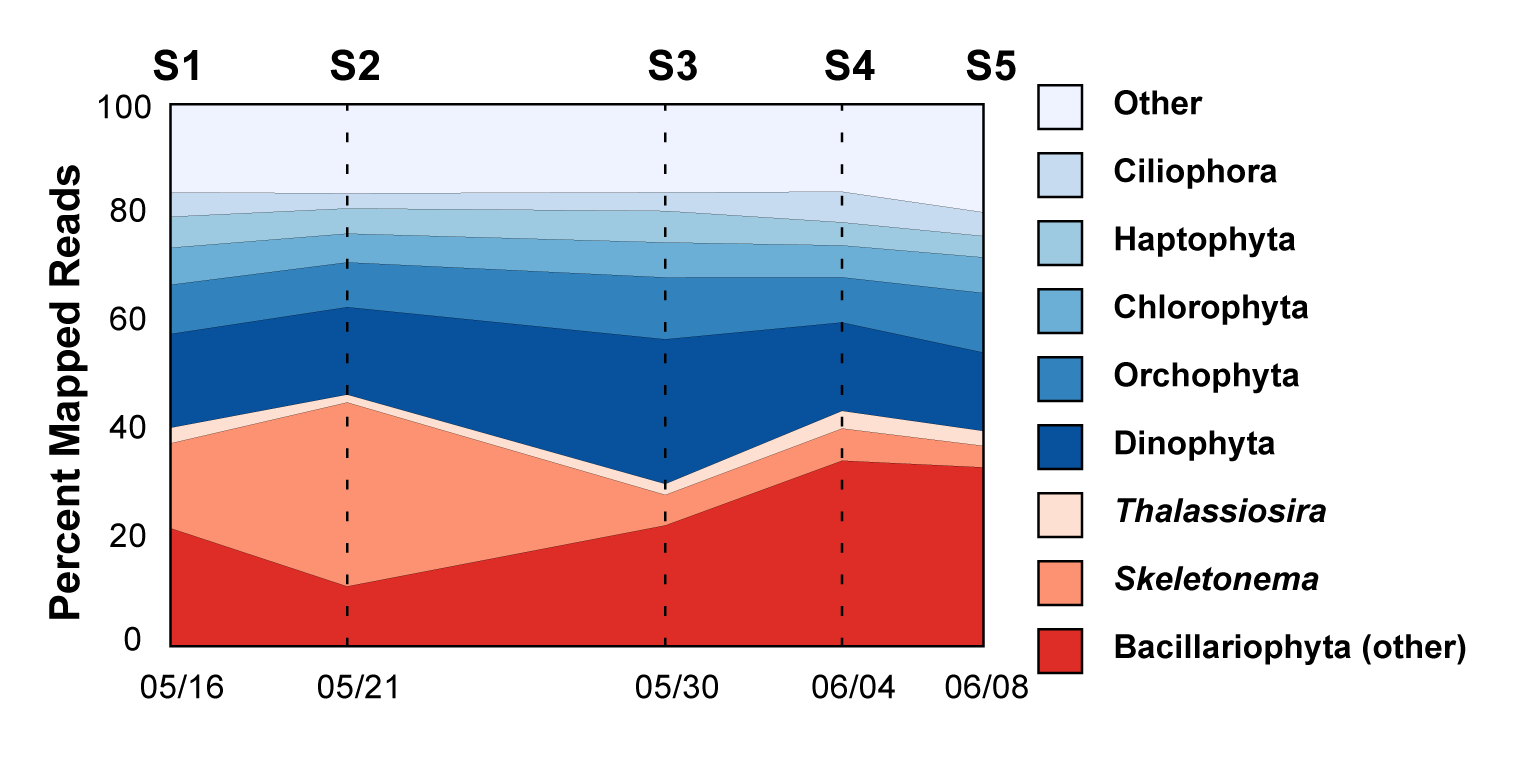
\includegraphics[width=1\textwidth]{Images/C3_Figure1_StackPlot.png}
    \caption[Taxonomic classification of reads across five field samples]{Taxonomic classification of RNA-seq paired end reads across the five field samples. Classification was determined by mapping to a database comprised of all publicly available transcriptomes through the Marine Microbial Eukaryotic Transcriptome Project (MMETSP) as of March 17, 2014.}
  \label{fig:c3f1}
\end{figure}

\subsection{Temporal plasticity in expressed metabolic capacity} 
Metatranscriptome short reads were mapped to transcriptomes that had been annotated with Kyoto Encyclopedia of Genes and Genomes (KEGG) orthology (KO) (\ref{DS31}), allowing the expression of KO gene families within a KEGG module (higher-level groupings of KO gene families into pathway or functional classifications) to be examined over time. Normalizing the expression of KEGG modules to the total KEGG annotated reads for each organism across time yielded the Quantitative Metabolic Fingerprint (QMF), which highlighted differences between the two species and differences across time for each species (Figure \ref{fig:c3f2}). A comparison of the total number of annotated genes falling into each of the KEGG modules revealed a close to one-to-one linear relationship (slope of 1.0948, $R^{2}=0.9123$) (Figure \ref{fig:a3f2}), indicating that the observed differences are not an artifact of gene distribution between organisms. The QMFs of the two organisms were distinct and there were significant shifts in the QMF of each species over time reflecting considerable plasticity in the expressed metabolic capacity (Figure \ref{fig:a3f3}). Central carbohydrate metabolism, carbon fixation, and other carbohydrate metabolism were some of the most highly expressed KEGG modules in the field for both \textit{Skeletonema} spp. and \textit{T. rotula}, though higher for \textit{Skeletonema} spp., where expression of these pathways peaked during S4 representing over 84\% of mapped KEGG reads (Figure \ref{fig:c3f2}). The largest global shift in KEGG module expression was seen in \textit{Skeletonema} spp. on S2 (Figure \ref{fig:a3f3}), when its density peaked at 11,520,000 cells L$^{-1}$. The S2 time point for \textit{Skeletonema} spp. had increased QMF signals in ATP synthesis, proteasome, and ubiquitin systems and decreased QMF signals in photosynthesis and carbon metabolism relative to other time points. For example, reads mapping in photosynthesis dropped by over an order of magnitude from 0.3-2.2\% of annotated transcripts in S1, S3-5 to 0.03\% during S2 (Figure \ref{fig:c3f2}). The temporal plasticity of transcript allocation to different aspects of metabolism for both species was striking and likely reflects the dynamic environment which they inhabit: an estuary, where the geochemistry is highly variable \citep{Nixon1995}.\par
Temporal plasticity in the KEGG module expression patterns, including a shift away from the expression of carbon fixation and photosynthesis suggests that the elevated \textit{Skeletonema} spp. cell numbers observed in S2 may have been after this diatom reached peak bloom biomass. A significant proportion of the KEGG modules expressed were classified as ribosomes (5-45\% for \textit{Skeletonema} spp. and 5-9\% for \textit{T. rotula}). \citet{Gifford2013} suggested that ribosomal protein expression correlates with growth rate. Applying this principle to these eukaryotic data suggests the growth rates for both \textit{Skeletonema} spp. and \textit{T. rotula} fluctuated, with peaks in growth rate occurring during S1 and S3 for \textit{Skeletonema} spp.. This pattern for \textit{Skeletonema} spp. did not track with the relative abundance of the organism, which peaked in the S2 sample, again suggesting that this sample was taken during the bloom decline. These growth dynamics cannot be fully resolved without a more detailed sample set.\par

% Figure 2
\begin{figure}[p!]
  \centerline{ 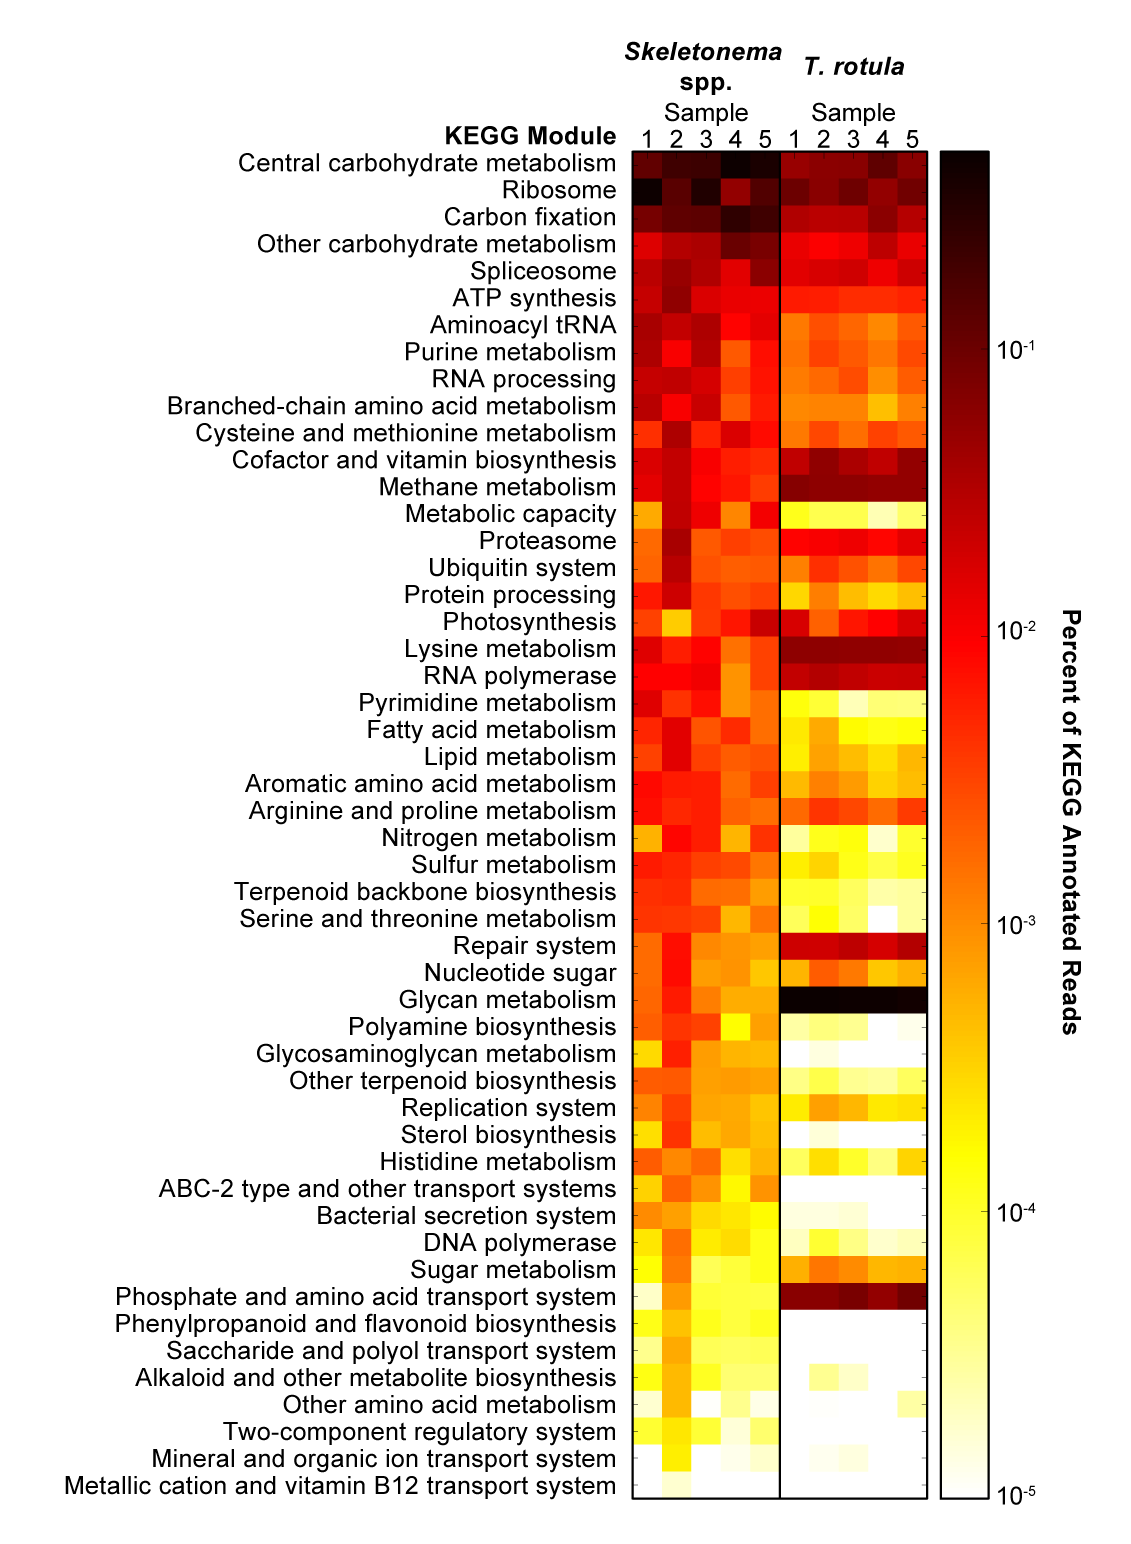
\includegraphics[width=1\textwidth]{Images/C3_Figure2_Heatmap_Hot.png}}
    \caption[Quantitative metabolic fingerprint across Narragansett Bay \textit{in situ} samples]{Quantitative metabolic fingerprint (QMF) depicting the relative expression of KEGG modules for \textit{Skeletonema} spp. and \textit{T. rotula} in Narragansett Bay across the five sampling time points (S1-S5). Color indicates the proportion of total reads mapping to each KEGG module relative to all KEGG annotated reads.}
  \label{fig:c3f2}
\end{figure}

\textit{Skeletonema} spp., the dominant diatom during the study period (Figure \ref{fig:c3f1}), had a higher proportion of transcripts related to growth relative to \textit{T. rotula}, such as those encoding aspects of carbon metabolism, N metabolism, sulfur metabolism, and lipid metabolism (Figure \ref{fig:c3f2}). Conversely, several KEGG modules were more highly expressed in \textit{T. rotula} compared to \textit{Skeletonema} spp., particularly those for glycan metabolism, phosphate and amino acid transport systems, and repair system modules (Figure \ref{fig:c3f2}). The majority of highly expressed KO modules (e.g. N metabolism) were based on moderate to high expression across several KO gene families, but, in some cases, the differences in expression at the module level were due to differences in the expression of a single KO gene family within the KEGG module. For example, the driver of the difference in the expression of glycan metabolism, which represented upwards of 41\% of all KEGG annotated reads for \textit{T. rotula} compared to less than 0.6\% for \textit{Skeletonema} spp., was primarily associated with the high expression of a putative UDP-N-acetylglucosamine-dolichyl-phosphate N-acetylglucosaminephosphotransferase (K01001). This was identified as a silaffin-like response gene associated with silica polymerization \citep{Shrestha2012}. Differences in silica metabolism may in part drive how the fundamental niche is segregated between these two diatoms. Taken together, the contrast in QMF between the two diatoms underscores the fundamental differences in expressed metabolic capacity that are present in these two co-occurring diatoms and highlights traits of a successful competitor (e.g. high expression of carbon metabolism).\par

\subsection{Species-specific resource utilization underpins physiological ecology}
KO gene families related to N and P metabolism were examined in the field samples to identify species-specific patterns in resource utilization. \textit{Skeletonema} spp. and \textit{T. rotula} both possess and express core pathways of N and P metabolism (such as the ornithine-urea cycle) (Figure \ref{fig:c3f3}). Expression of these individual KO gene families was temporally variable, as was observed with the expression of KEGG Modules, but related enzymes in a pathway exhibited a coordinated response (Figure \ref{fig:c3f3}). For example, the nitrate transporter (K02575), nitrate reductase (K10534), and nitrite reductase (K00366), in \textit{Skeletonema} spp. all had peak expression in S2 (Figure \ref{fig:c3f3}). \textit{Skeletonema} spp. and \textit{T. rotula} share pathway homologs, including the same suite of N transporters (ammonium: AMT, nitrate: NRT, amino acid: AAPJ), but these genes often had disparate patterns of expression between the two species (Figure \ref{fig:c3f3}). \textit{Skeletonema} spp., the more abundant diatom, had high expression of KO gene families associated with the acquisition of nitrate and ammonia that were particularly amplified during the S2 bloom event. \textit{T. rotula} had low expression of both of those transporters but high expression of a general amino acid transporter (Figure \ref{fig:c3f3}). Amino acid transport \citep{North1972} and nitrate transport \citep{Serra1978} has previously been found to inversely correlate with intracellular nitrate concentration in the cell or the presence of ammonia in the media. Yet, here, two closely related diatoms, existing in the same parcel of water and the same nutrient environment, are expressing genes to access different pools of dissolved N. Similar to nitrate transport, there was high expression of nitrate/ nitrite reductase KO gene families in \textit{Skeletonema} spp., whereas \textit{T. rotula} appears to possess a different N reduction metabolism. This is observed in a KO gene family that is absent from the reference transcriptome of \textit{Skeletonema} spp.: hydroxylamine reductase (Figure \ref{fig:c3f3}). This gene has been found in the genomes of both \textit{T. pseudonana} and \textit{P. tricornutum}, and is thought to have been acquired via lateral transfer from bacteria \citep{Bowler2008}. The enzyme may potentially aid redox balancing and electron cycling from nitrate reduction \citep{Allen2008}. While the absence of this gene in \textit{Skeletonema} spp., has not been definitively shown, the marked high expression of this gene in \textit{T. rotula} suggests that this gene product represents a potential point of segregation in the metabolic capacity of these two species. Together, these data suggest that these species have disparate strategies for acquiring N and this may in part drive the relative success of \textit{Skeletonema} spp. over the sample period.\par

%Figure 3

\begin{figure}[p!]
  \centering
    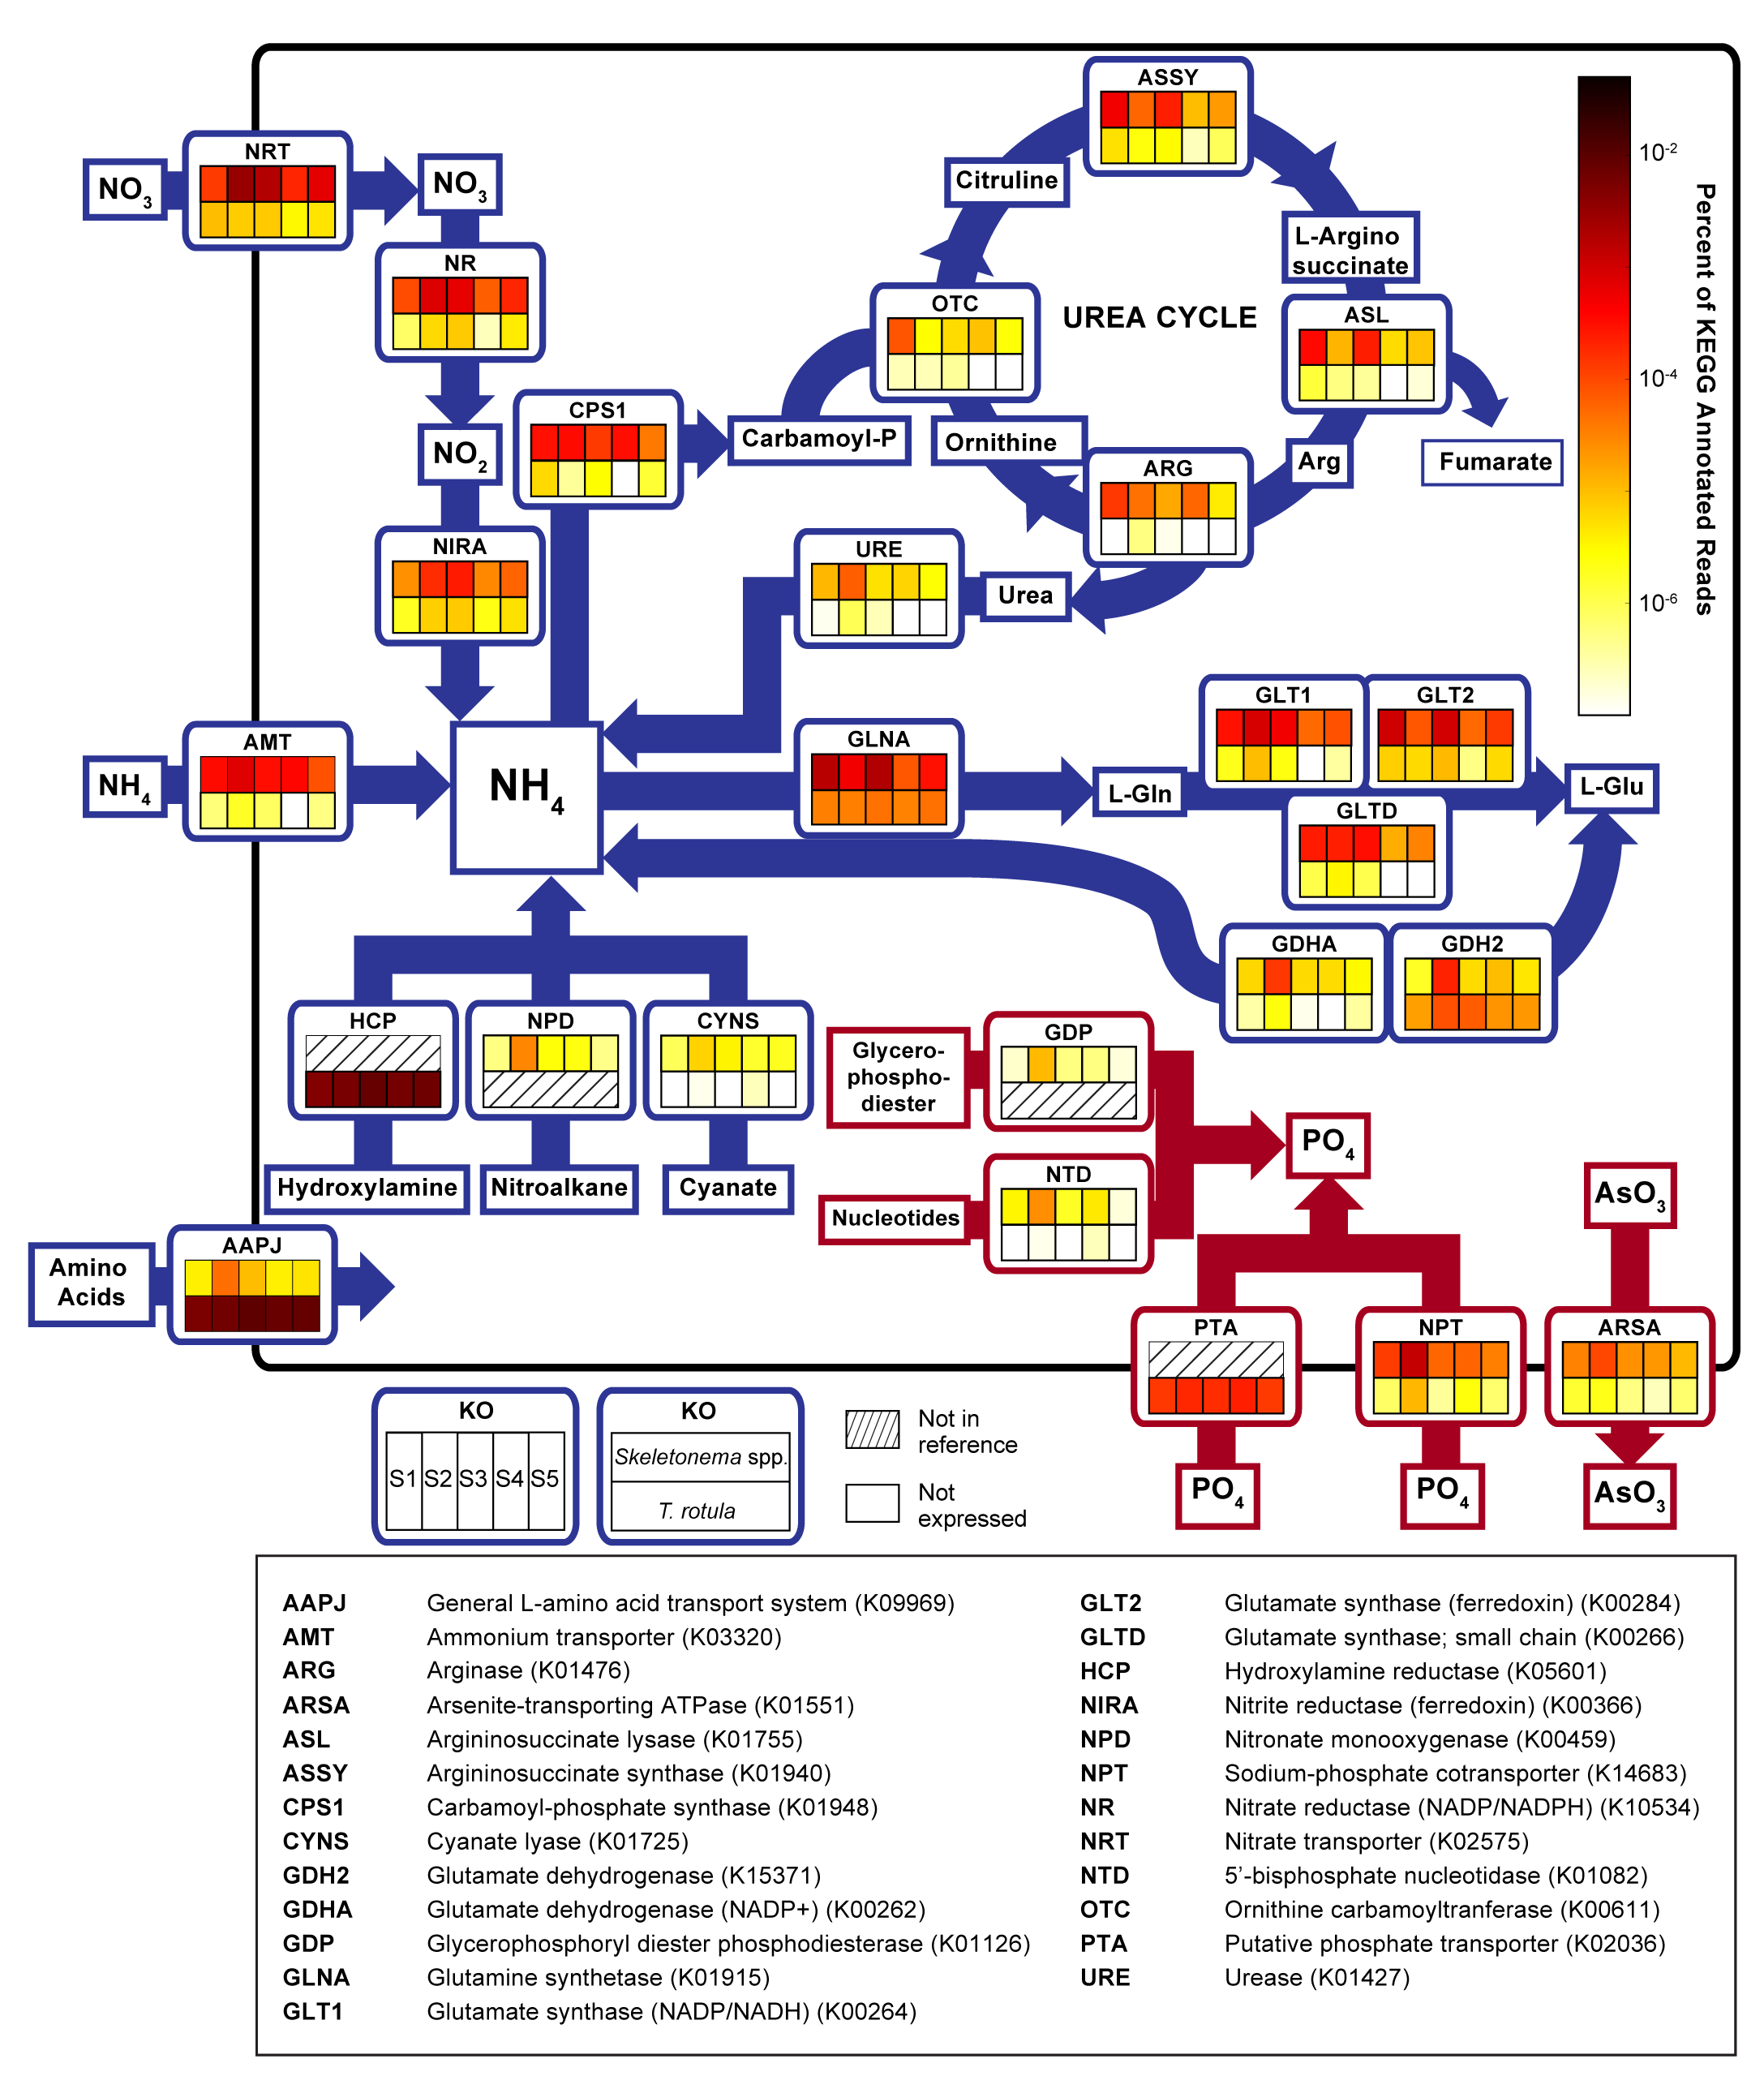
\includegraphics[width=1\textwidth]{Images/C3_Figure3_CellHeatmap_Hot.png}
    \caption[Modulation of nitrogen and phosphorus pathways in the field]{Schematic cell model depicting the relative expression of KO gene families associated with nitrogen (N) and phosphorus (P) metabolic pathways for \textit{Skeletonema} spp. and \textit{T. rotula} in Narragansett Bay across the five sampling time points (S1-S5). Color indicates the proportion of total reads mapping to each KEGG module relative to all KEGG annotated reads.}

  \label{fig:c3f3}
\end{figure}



While N has been observed to be a primary nutritional driver in Narragansett Bay \citep{Nixon1995,Smayda1974,Sakshaug1977}, P may also drive the dynamics of these two diatoms. \textit{Skeletonema} spp. shows elevated expression of a sodium phosphate cotransporter (NPT), again with peak expression during S2 (bloom). \textit{T. rotula} does express the NPT as highly, but by comparison has a much higher transcript count for a putative P transporter (PTA), that is not detected in \textit{Skeletonema} spp. (Figure \ref{fig:c3f3}). These transporters may have different kinetic properties that allow the two species to diverge in their PO$_4$ uptake strategies.  Genes associated with the scavenging of P from organic molecules, such as glycerophosphoryl diester phosphodiesterase (GDP), also suggest differences in expressed metabolic capacity between the two species. GDP may be associated with exogenous metabolism of dissolved organic P (DOP) or internally in the cleaving of P from lipids \citep{VanMooy2009, Dyhrman2012}. The expression of GDP by \textit{Skeletonema} spp., with peak around S2, and apparent absence of this transcript in \textit{T. rotula} suggests \textit{Skeletonema} spp. may be accessing a pool of DOP that is not being utilized by \textit{T. rotula}. In \textit{T. pseudonana}, related transcripts are tightly linked to concomitant changes in the proteome and biochemical activities \citep{Dyhrman2012}.  If these transcriptional patterns are linked to similar changes in activities, then these insights suggest that there is a fundamental difference in the metabolic capacity being expressed in the same environment by the two diatoms.  \textit{Skeletonema} spp. is both actively taking up PO$_4$ and hydrolyzing organic sources, where as \textit{T. rotula} is not hydrolyzing DOP and is taking up inorganic PO$_4$ by a different mechanism.  In summary, these data suggest that these two diatoms have unique metabolic capacity for the utilization of specific forms of N and P. Such disparate resource utilization potential could be a niche-defining feature that underpins diatom diversity as well as the ``winner-loser'' dynamic observed here with the differences in cell abundance between the species.\par
\subsection{Identification and modulation of resource responsive genes \textit{in situ} highlights species-specific differences}
To identify and quantitatively track resource responsive (RR) genes \textit{in situ}, incubation experiments were used to examine species-specific transcriptional responses to shifts in N:P ratios. Comparing the expression patterns between like nutrient treatments (+N versus -N and +P versus -P) for each of the organisms enabled the statistical identification of a suite of RR genes \citep{Wu2010} and stable reference genes \citep{Alexander2012}. RR gene counts were normalized to the stable reference genes (Figure \ref{fig:a3f4}) resulting in stable gene normalized counts ($SGNC$). Calculation of a $SGNC$ is similar in concept to reference gene normalization done in qRT-PCR \citep{Bustin2000} or metatranscriptome studies of prokaryotes \citep{McCarren2010}, with the added value of not having to rely on reference genes from model diatoms.\par
Of the transcripts expressed at greater than 2 tags per million (TPM) for at least one treatment, 24.5\% and 17.9\% were identified as RR by being significantly up or down-regulated between N or P treatments for \textit{Skeletonema} spp. and \textit{T. rotula}, respectively (\ref{DS32}, Table \ref{tab:a3t3}). As is common with phytoplankton studies \citep{Marchetti2012a}, the majority of the RR genes do not have a KEGG annotation (Figure \ref{fig:a3f4}A). The portion of the RR gene set annotated with KEGG ontology for \textit{Skeletonema} spp. and \textit{T. rotula} revealed that, relative to the full KEGG profile, genes comprising genetic information processing associated with replication (encompassing ribosomes, nucleotide replication and processing) were underrepresented for both organisms in the RR set (Figure \ref{fig:a3f5}). By contrast, the RR sets were enriched for energy, carbohydrate, and lipid metabolism, which encompass pathways known to be associated with the metabolism of N and P (Figure \ref{fig:c3f4}A, Figure \ref{fig:a3f5}). Specific genes in this set included, but were not limited to, those associated with N assimilation (e.g. glutamate dehydrogenase, glutamine synthase, nitrate reductase), DON utilization (e.g. urease, aminopeptidase, amino-acid transport system), P scavenging (e.g. phosphate transporter, sodium phosphate cotransporter) and DOP utilization (e.g. phosphatases) (\ref{DS32}). A number of these genes have been shown to be N or P responsive in transcriptional studies with cultures of the diatom \textit{T. pseudonona} \citep{Dyhrman2012, Bender2014}, and transporters, and enzymes for the processing of organic N or P, as observed here, are well known to be resource responsive in many phytoplankton \citep{Dyhrman2012, Wurch2011, Dyhrman2006, Bruhn2010}. Overall, these genes demonstrated patterns of regulation \textit{in situ} (Figure \ref{fig:c3f4}B, Figure \ref{fig:a3f6}) similar to what has been observed in culture \citep{Dyhrman2012, Bender2014}. In the incubations, the sodium-phosphate cotransporter (NPT) was significantly up-regulated in the -P treatment for both species (Figure \ref{fig:c3f4}B), which is consistent with P regulation of a \textit{T. pseudonana} NPT homolog (Thaps\_24435) observed in culture experiments (56). Nitrate reductase, which has been shown to be regulated by N in \textit{T. pseudonana} (Thaps\_25299) \citep{Bender2012}, was up-regulated in -N for \textit{T. rotula}, but not \textit{Skeletonema} spp. (Figure \ref{fig:a3f6}). In fact, members of this large gene family (Figure \ref{fig:a3f7}) showed disparate regulation in both species (Figure \ref{fig:a3f6}).  These data demonstrate that the use of nutrient amendments is robust for normalizing and identifying N and P responsive genes in the field that are consistent with known signals, but also point to the value of \textit{in situ} analyses, as application of a priori knowledge about regulation from model diatoms could lead to misinterpretations.\par

% Figure 4


\begin{figure}[p!]
  \centering
    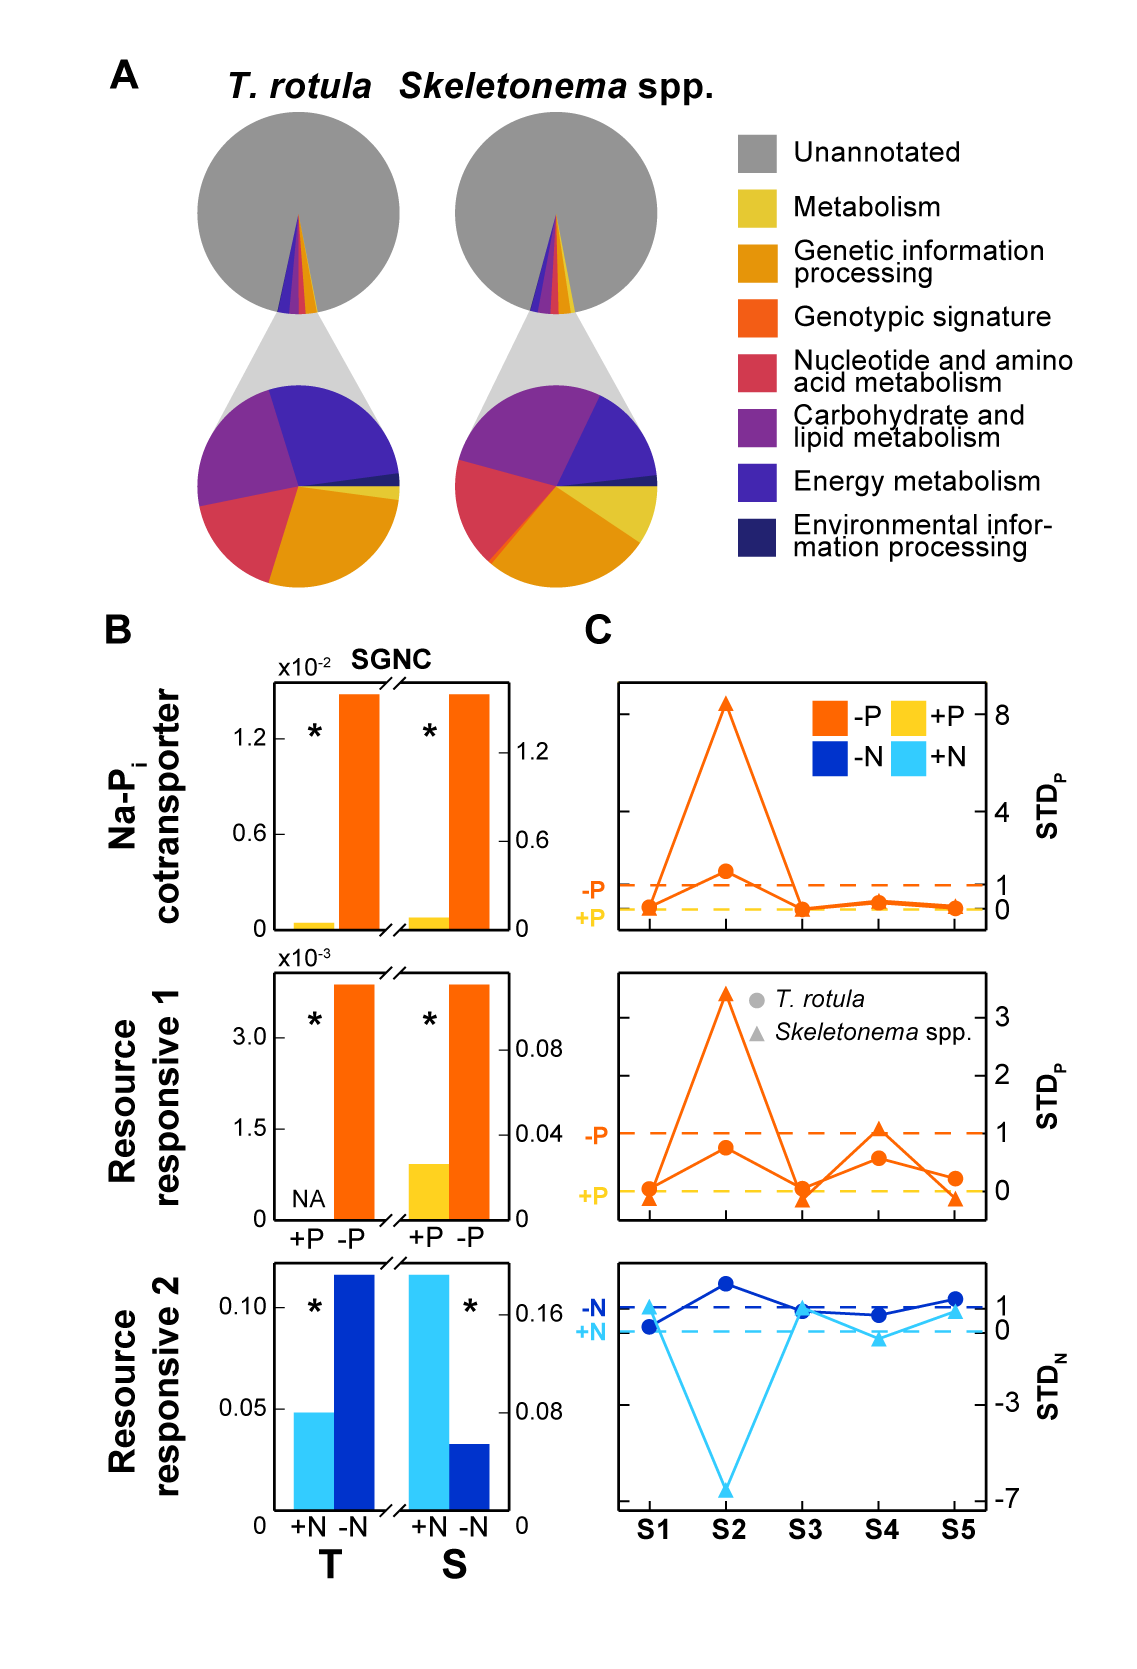
\includegraphics[width=.65\textwidth]{Images/C3_Figure4_BarLinePlots.png}
    \caption[Functional composition of resource-responsive gene set]{Functional composition of the resource-responsive (RR) gene sets for \textit{T. rotula} and \textit{Skeletonema} spp. (A), the relative expression in the incubation samples (B) and standardized transcriptional differentiation (STD) scores (C) for a known P-responsive gene, sodium-phosphate cotransporter, and two novel RR gene families. (A) The RR gene sets were identified through cross comparison of like-nutrient incubations (i.e. +N vs. -N and +P vs. -P), using ASC (fold change = 2, post-$p > 0.95$) (57). The relative functional categorization of the RR gene set for \textit{T. rotula} and \textit{Skeletonema} spp. based on KEGG ontology as assigned by KAAS is depicted at the module-level relative to the portion unannotated with KEGG. (B) Expression pattern in stable gene normalized counts ($SGNC$) of the genes from the associated gene cluster from \textit{T. rotula} (T) and \textit{Skeletonema} spp. (S) plotted in related incubations (i.e. novel P-responsive shows expression from +P and -P incubations). Asterisk indicates significance between pair-wise comparisons (fold change = 2, post$-p > 0.95$) (57). (C) $STD$ scores plotted across the five sample points showing $STD_P$ for the P-significant genes and $STD_N$ for the N-significant genes. Dashed horizontal lines at 0 and 1 indicate the +P/+N and -P/-N for corresponding significant genes.} 
  \label{fig:c3f4}
\end{figure}

Of the RR gene sets for \textit{Skeletonema} spp. and \textit{T. rotula}, only 17.7 and 12.7\% of the genes, respectively, were annotated with KEGG ontology (Figure \ref{fig:c3f4}A). Identifying differentially regulated genes \textit{in situ} through experimental manipulations allowed the expression patterns of genes to be tracked even when their function was unknown. As an example, two RR gene families were identified with homologs in \textit{Skeletonema} spp. and \textit{T. rotula} (Figure \ref{fig:c3f4}B, Figure \ref{fig:a3f7}). RR1 was up-regulated in -P compared to +P for both species (Figure \ref{fig:c3f4}B). Homologs from RR1 were also identified in other diatom genomes (Fracy\_268075, Phatr\_19661, Psemu\_246578, Psemu\_319824, Thaps\_32459) (Figure \ref{fig:a3f7}). Annotations for these genes were limited, though Fracy\_268075 was identified as possibly involved in intracellular trafficking, secretion, or vesicular transport; suggesting these proteins may be involved in poly-P metabolism \citep{Ogawa2000}. RR2 demonstrated significantly different patterns of regulation in the two species: up-regulated in -N compared to +N for \textit{T. rotula} but down-regulated in -N compared to +N for \textit{Skeletonema} spp. (Figure \ref{fig:c3f4}B). A homolog from RR2 was identified in \textit{T. pseudonana} (Thaps\_22648) (Figure \ref{fig:a3f7}) and was poorly characterized, with the best BLAST hit to a human dentin sialophosphoprotein. This suggests RR2 could be associated with biomineralization.\par
To enable cross-comparison of the RR genes between species, their expression was put into a greater metabolic context by proportionalizing the expression in the field to the transcriptional range observed in the incubations with extremes in the N:P ratio. This technique is similar in concept to targeted assays using qRT-PCR to compare expression patterns between species in culture \citep{Kang2009}. Briefly, the $SGNC$ of a gene in the field was bounded by the $SGNC$ from each of the nutrient treatments to yield the standardized transcriptional differentiation score for both N ($STD_N$) and P ($STD_P$) (Figure \ref{fig:c3f4}C). The $STD$ score was used to directly compare expression relative to its maximum and minimum capacity where values of $STD \geq 1$ indicate signals are similar to the deplete condition, and values of $STD \leq 0$ indicate similarity to the replete condition. The $STD_N$ and $STD_P$ were plotted for genes from the NPT and the two highlighted RR gene families, over the time-series (Figure \ref{fig:c3f4}C). The NPT for both \textit{Skeletonema} spp. and \textit{T. rotula} showed elevated expression during S2. RR1, which was also identified as significantly expressed in -P compared to +P, also showed elevation during S2 (the bloom day). The expression of RR1, however, was also elevated on S4 for both diatoms, which was not seen for the NPT. However, $STD_P >1$ for \textit{Skeletonema} spp. indicating a far more P deficient response in \textit{Skeletonema} spp. compared to \textit{T. rotula}, which never demonstrated P-sensitive expression in the field comparable to that observed in the -P incubations (Figure \ref{fig:c3f4}C). RR2 showed different patterns of expression across time for both species. Most interestingly, perhaps, was the low $STD_N$ score for \textit{Skeletonema} spp. during its bloom period indicating that the RR2 expression was more similar to the +N treatment, whereas the $STD_N$ for \textit{T. rotula} was greater than one suggesting that expression was more similar to the -N treatment (Figure \ref{fig:c3f4}C). These three, targeted examples suggest that during the large bloom of \textit{Skeletonema} spp., \textit{Skeletonema} spp. was expressing genes in pattern more similar to the -P and +N treatments, while the expression of \textit{T. rotula} was more similar only to the -N treatment. Notably, these are orthogonal patterns associated with the same environment. \par
% Figure 5
\begin{figure}[p!]
  \centering
    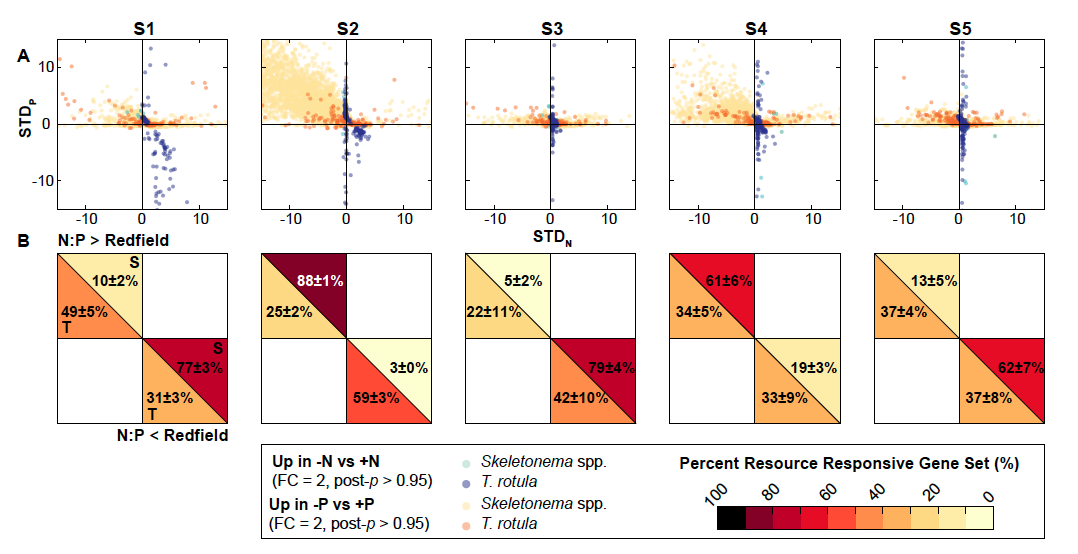
\includegraphics[width=1\textwidth]{Images/C3_Figure5_Quadrants.png}
    \caption[Evolution of resource-responsive (RR) gene partitioning over time in Narragansett Bay]{Evolution of resource-responsive (RR) gene partitioning over time in Narragansett Bay for \textit{T. rotula} and \textit{Skeletonema} spp.. (A) The stable gene normalized field signal for each gene identified as significantly (2-fold change, post-p > 0.95) up-regulated in -P vs. +P for \textit{Skeletonema} spp. (yellow) and \textit{T. rotula} (orange) and in -N vs. +N for \textit{Skeletonema} spp. (cyan) and \textit{T. rotula} (dark blue) were proportionalized relative to the expression for those genes in nutrient incubations, yielding the $STD_N$ and $STD_P$ for each gene. These data are plotted for Sample 1 through Sample 5. (B) The proportion of identified RR genes falling into the N:P > Redfield and N:P < Redfield quadrants for \textit{T. rotula} (T) and \textit{Skeletonema} spp. (S).}

  \label{fig:c3f5}
\end{figure}

The $STD_N$ and $STD_P$ for all of the RR genes were calculated (\ref{DS32}) to expand upon the single gene analyses above. The RR genes were plotted based on the $STD_N : STD_P$ (Figure \ref{fig:a3f8}) to examine how similar the pattern was to the incubation N:P ratio (Figure \ref{fig:c3f5}A, Figure \ref{fig:a3f9}). Redfield regimes have historically been used to characterize different aquatic environments based on the ratio of nutrient resources required for growth. For example, a Redfield ratio of N:P = 16, here called “Redfield”, would predict neither P nor N limitation. As expected, RR genes identified as N-regulated genes fall primarily into the N:P < Redfield quadrant and P-regulated genes fall primarily into the N:P > Redfield quadrant for both \textit{Skeletonema} spp. and \textit{T. rotula} (Figure \ref{fig:c3f5}A). Observing patterns in distribution of these genes across time, S2 stands out amongst the time points, where a significant (88\%) proportion of the P-regulated genes from \textit{Skeletonema} spp. move far into the N:P > Redfield quadrant (Figure \ref{fig:c3f5}A). This N:P > Redfield physiology is consistent with the single gene analyses (Figure \ref{fig:c3f4}C) and suggests P availability may have constrained \textit{Skeletonema} spp. populations during the bloom sample (S2). Conversely, a large proportion (59\%) of the N-regulated genes in \textit{T. rotula} move into the N:P < Redfield quadrant (Figure \ref{fig:c3f5}A) consistent with the divergent responsiveness of RR2 observed for \textit{T. rotula} compared to \textit{Skeletonema} spp. (Figure \ref{fig:c3f4}C). In fact, with the exception of S4 and S5 where \textit{T. rotula} had even distribution between the N:P > Redfield and N:P < Redfield quadrants, the two species always showed statistically significant (Tukey HSD analysis ($p<0.05$)) orthogonal responses in the distribution of the RR gene set across the two quadrants (Figure \ref{fig:c3f5}B, Figure \ref{fig:a3f10}). These patterns combined with the temporal variability in gene expression patterns indicate a finely tuned response to the environment, which is distinctive for each diatom species. Although there are many potential controls on diatom dynamics in Narragansett Bay, including top-down processes like predation \citep{Martin1970, Lawerence2012}, these patterns of resource responsive gene expression suggest the presence of bottom-up nutrient control on diatom population dynamics in Narragansett Bay.\par

This work addresses fundamental knowledge gaps in how phytoplankton species are able to co-occur while they compete for the same basic resources. Co-occurring diatoms appear to have different functional capabilities in N and P metabolism, and this metabolic potential is modulated in field populations in a distinctive way for each diatom. These findings suggest that differential resource partitioning is occurring between these two diatoms \textit{in situ}. Such resource partitioning could facilitate the vast diversity of the phytoplankton and the structure, function, and productivity of aquatic ecosystems. In culture studies, resource-related transcriptional changes have been shown to be tightly choreographed with changes in proteins, activities, and biochemical pools (56, 62, 69). If further work were able to similarly link the transcriptional patterns observed here with changes in enzymatic activities or uptake rates, then shifts in the RR gene sets may reflect aspects of the realized niche and how it differs between these two species. These detailed, \textit{in situ} transcriptional comparisons would not have been possible without proportionalization to metabolic capacity (STD), which provides a quantitative means to directly compare transcriptional patterns between species. This approach could be applied to other systems, organisms, or environmental parameters to identify responsive genes and proportionalize their expression, with the aim of answering similar questions about how co-occurring species adjust their cellular physiology to partition their niche space.\par

